\documentclass{article}

\usepackage{fancyhdr}
\usepackage{extramarks}
\usepackage{amsmath}
\usepackage{amsthm}
\usepackage{amsfonts}
\usepackage{tikz}
\usepackage[plain]{algorithm}
\usepackage{algpseudocode}
\usepackage{enumerate}
\usepackage{amssymb}

\usetikzlibrary{automata,positioning}

%
% Basic Document Settings
%

\topmargin=-0.45in
\evensidemargin=0in
\oddsidemargin=0in
\textwidth=6.5in
\textheight=9.0in
\headsep=0.25in

\linespread{1.1}

\pagestyle{fancy}
\lhead{\hmwkAuthorName}
\chead{\hmwkClass\ (\hmwkClassInstructor\ \hmwkClassTime): \hmwkTitle}
\rhead{\firstxmark}
\lfoot{\lastxmark}
\cfoot{\thepage}

\renewcommand\headrulewidth{0.4pt}
\renewcommand\footrulewidth{0.4pt}

\setlength\parindent{0pt}

%
% Create Problem Sections
%

\newcommand{\enterProblemHeader}[1]{
    \nobreak\extramarks{}{Problem \arabic{#1} continued on next page\ldots}\nobreak{}
    \nobreak\extramarks{Problem \arabic{#1} (continued)}{Problem \arabic{#1} continued on next page\ldots}\nobreak{}
}

\newcommand{\exitProblemHeader}[1]{
    \nobreak\extramarks{Problem \arabic{#1} (continued)}{Problem \arabic{#1} continued on next page\ldots}\nobreak{}
    \stepcounter{#1}
    \nobreak\extramarks{Problem \arabic{#1}}{}\nobreak{}
}

\setcounter{secnumdepth}{0}
\newcounter{partCounter}
\newcounter{homeworkProblemCounter}
\setcounter{homeworkProblemCounter}{1}
\nobreak\extramarks{Problem \arabic{homeworkProblemCounter}}{}\nobreak{}

%
% Homework Problem Environment
%
% This environment takes an optional argument. When given, it will adjust the
% problem counter. This is useful for when the problems given for your
% assignment aren't sequential. See the last 3 problems of this template for an
% example.
%
\newenvironment{homeworkProblem}[1][-1]{
    \ifnum#1>0
        \setcounter{homeworkProblemCounter}{#1}
    \fi
    \section{Problem \arabic{homeworkProblemCounter}}
    \setcounter{partCounter}{1}
    \enterProblemHeader{homeworkProblemCounter}
}{
    \exitProblemHeader{homeworkProblemCounter}
}

%
% Homework Details
%   - Title
%   - Due date
%   - Class
%   - Section/Time
%   - Instructor
%   - Author
%

\newcommand{\hmwkTitle}{Tutorial 7}
\newcommand{\hmwkDueDate}{March 9, 2021}
\newcommand{\hmwkClass}{CZ2003}
\newcommand{\hmwkClassTime}{SS3}
\newcommand{\hmwkClassInstructor}{Assoc Prof Alexei Sourin}
\newcommand{\hmwkAuthorName}{\textbf{Pang Yu Shao}}
\newcommand{\hmwkAuthorID}{\textbf{U1721680D}}

%
% Title Page
%

\title{
    \vspace{2in}
    \textmd{\textbf{\hmwkClass:\ \hmwkTitle}}\\
    \normalsize\vspace{0.1in}\small{Due\ on\ \hmwkDueDate\ at 10:30am}\\
    \vspace{0.1in}\large{\textit{\hmwkClassInstructor\ - \hmwkClassTime}}
    \vspace{3in}\\
    \hmwkAuthorName\\
    \hmwkAuthorID
}

\date{08/03/2021}

\renewcommand{\part}[1]{\textbf{\large Part \Alph{partCounter}}\stepcounter{partCounter}\\}

%
% Various Helper Commands
%

% Useful for algorithms
\newcommand{\alg}[1]{\textsc{\bfseries \footnotesize #1}}

% For derivatives
\newcommand{\deriv}[1]{\frac{\mathrm{d}}{\mathrm{d}x} (#1)}

% For partial derivatives
\newcommand{\pderiv}[2]{\frac{\partial}{\partial #1} (#2)}

% Integral dx
\newcommand{\dx}{\mathrm{d}x}

% Alias for the Solution section header
\newcommand{\solution}{\textbf{\large Solution}}

% Probability commands: Expectation, Variance, Covariance, Bias
\newcommand{\E}{\mathrm{E}}
\newcommand{\Var}{\mathrm{Var}}
\newcommand{\Cov}{\mathrm{Cov}}
\newcommand{\Bias}{\mathrm{Bias}}

\begin{document}

\maketitle

\pagebreak

\begin{homeworkProblem}
    Consider a 2D object defined implicitly by\\
    \(max(1-(x-1)^2-y^2, min(min(x-1,2-x,y,2-y), -(0.25 - (x-2)^2 - (y-2)^2))) \geq 0\)
    \begin{enumerate}[i]
        \item Draw a diagram to show the hierarchical representation of the object.
        \item Find the minimum axis-aligned bounding rectangle of the object.
    \end{enumerate}
    \begin{figure}[H]
        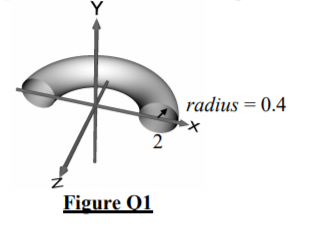
\includegraphics[width=6cm]{fig/q1.PNG}
        \centering
    \end{figure}
    

    \textbf{Solution}\\
    Part i:\\
    We can see that the 2D object is made up of 3 main components:
    \begin{enumerate}
        \item A Big Circle, defined by \(1 - (x-1)^2 - y^2 \geq 0\)
        \item A Rectangle, defined by \(min(x-1, 2-x, y, 2-y) \geq 0\), which is made of
        \subitem \(x - 1 \geq 0\)
        \subitem \(2 - x \geq 0\)
        \subitem \(y \geq 0\)
        \subitem \(2 - y \geq 0\) 
        \item A Small Circle, defined by \(0.25 - (x-2)^2 - (y-2)^2 \geq 0\) (subtracted from the rectangle)
    \end{enumerate}
    \begin{figure}[H]
        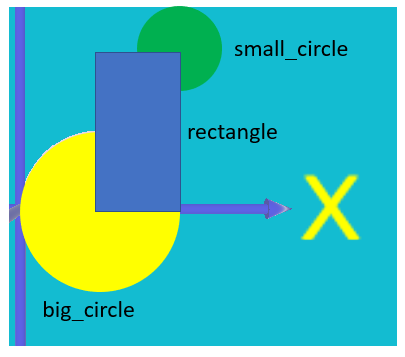
\includegraphics[width=6cm]{fig/q1i.PNG}
        \centering
    \end{figure}

    Therefore, a DAG can be used as the hierarchical representation as shown below:

    \begin{figure}[H]
        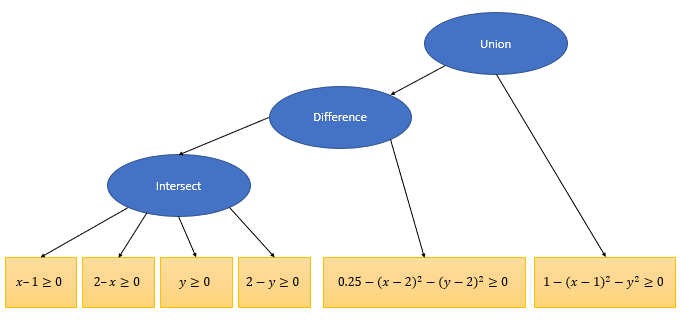
\includegraphics[width=15cm]{fig/q1idag.PNG}
        \centering
    \end{figure}
    Part ii:\\
    The minimum axis-aligned bounding rectangle of the object is shown below:
    \begin{figure}[H]
        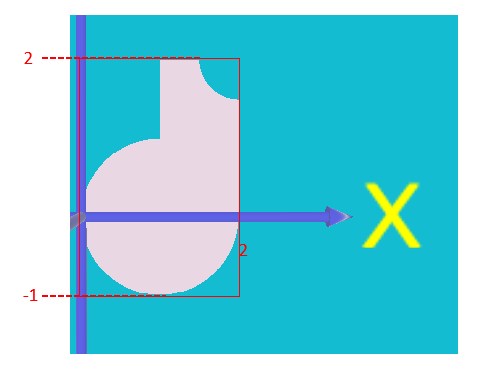
\includegraphics[width=15cm]{fig/q1ii.PNG}
        \centering
    \end{figure}

    Therefore, the bounding box \textbf{size} can be given as \((2,3)\), with the bounding box \textbf{location} being \((1, 0.5)\)
    

    

\end{homeworkProblem}
\pagebreak
\begin{homeworkProblem}
    With reference fo Figure Q2, suggest a database organization for a virtual city containing a 
    factory, an office, houses and trees. The organization should be hierarchical and does not have duplication
    in the primitive level.
    \begin{figure}[H]
        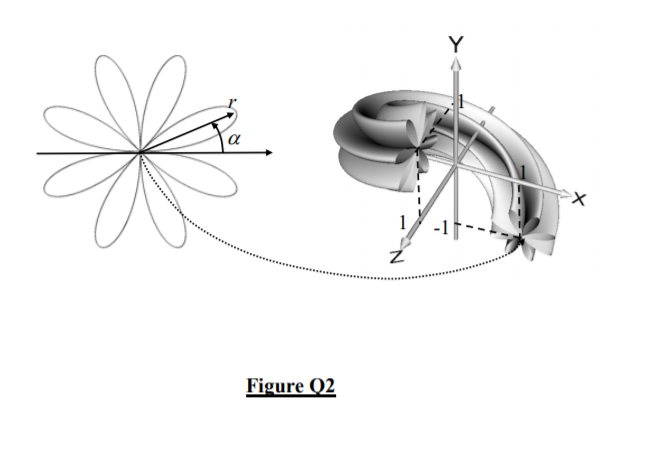
\includegraphics[width=8cm]{fig/q2.PNG}
        \centering
    \end{figure}

    \textbf{Solution}\\
    For this question, spacially-partitioned organization is used for efficient rendering.
    The virtual city is divided into 4 tiles as shown below:\\
    \begin{figure}[H]
        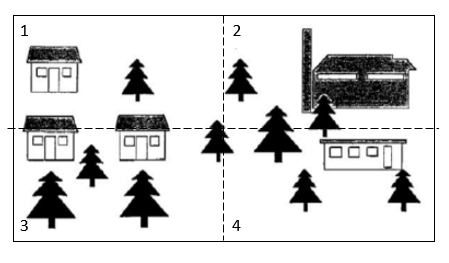
\includegraphics[width=6cm]{fig/q2div.PNG}
        \centering
    \end{figure}
    Therefore, the organization can be shown with the following DAG:
    \begin{figure}[H]
        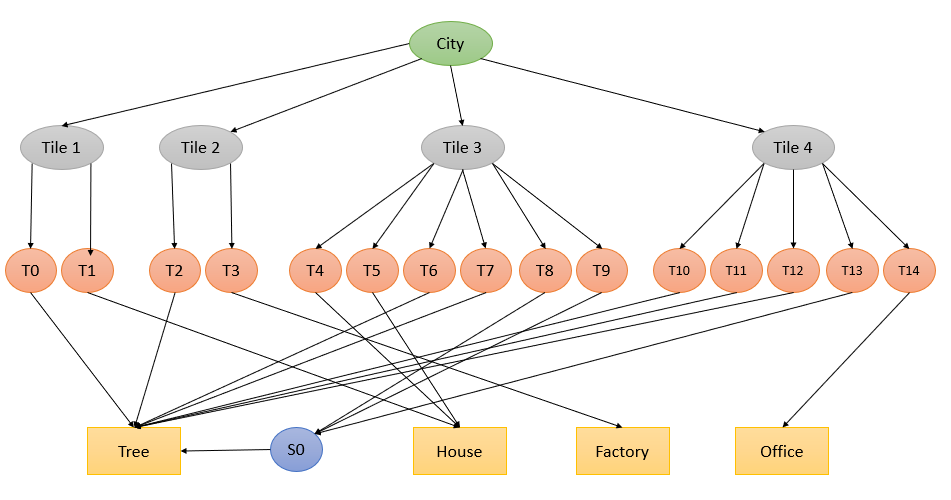
\includegraphics[width=15cm]{fig/q2ans.PNG}
        \centering
    \end{figure}
\end{homeworkProblem}

\pagebreak
\begin{homeworkProblem}
    Propose how to implement parametrically a continuous level-of-detail for an 
    ellipsoid defined by parametric equations
    \begin{displaymath}
        x = 1 + cos\phi cos\theta\ \ \ -\pi/2 \leq \phi \leq \pi/2
    \end{displaymath}
    \begin{displaymath}
        y = 2 + 2cos\phi cos\theta\ \ \ \ 0\leq \theta \leq 2\pi
    \end{displaymath} 
    \begin{displaymath}
        z = 3 + 3sin\phi
    \end{displaymath} 

    \textbf{Solution}\\
    A continuous LOD can be implemented by sampling \(\phi\) and \(\theta\) based on the 
    distance from the observer to the ellipsoid.

    The sampling for \(\phi\) can be defined as:
    \begin{displaymath}
        \phi = -\frac{\pi}{2} + \delta \cdot i
    \end{displaymath}

    The sampling for \(\theta\) can be defined as 
    \begin{displaymath}
        \theta = \delta \cdot j
    \end{displaymath}

    where \(\delta\) is a function of distance, \(\delta = \delta(d)\).\\

    For instance, it can be defined as:
    \begin{displaymath}
        \delta(d) = c*d + \epsilon
    \end{displaymath}
    Where \(c\) and \(\epsilon\) are two constants

\end{homeworkProblem}

\pagebreak
\begin{homeworkProblem}
    With reference to Figure Q4, a 3D object is defined implicitly by:
    \begin{displaymath}
        min(z, min(1-z, 1-\frac{x^2}{4}-y^2)) \geq 0
    \end{displaymath}
    \begin{enumerate}[i]
        \item Find the minimum axis-aligned bounding volume of the object.
        \item Propose reasonable resolutions for visualizing this object.
    \end{enumerate}
    \begin{figure}[H]
        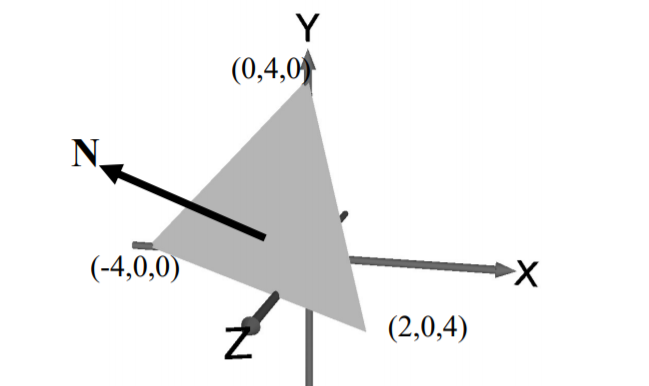
\includegraphics[width=10cm]{fig/q4.PNG}
        \centering
    \end{figure}

    \textbf{Solution}\\
    Part i:\\
    First, we find the limits of the 3D object in XYZ:\\
    Max X: +2\\
    Min X: -2\\
    Max Y: +1\\
    Min Y: -1\\
    Max Z: 1\\
    Min Z: 0\\
    Therefore, Bounding Box Size can be obtained with the following:\\
    \(BBSize = (2-(-2)\ \ 1-(-1)\ \  1-0) = \mathbf{(4\ \ 2\ \ 1)}\) \\
    Bounding Box Position can be obtained with the following:\\
    \(BBPosition = ((2+(-2))/2\ \ (1+(-1))/2\ \  (1+0)/2) = \mathbf{(0\ \ 0\ \ 0.5)}\)\\\\
    \newpage
    Part ii:\\\\
    To replicate the figure with the distance shown in Q4, a sampling resolution of \(\mathbf{(150\ \ 150\ \ 50)}\)
    is reasonable for visualizing it:
    \begin{figure}[H]
        \includegraphics[width=15cm]{fig/q4iia.PNG}
        \centering
    \end{figure}

    However, when zoomed in, the interpolations can be seen and the edges of the object appear jagged. Therefore a higher sampling resolution would be required:
    \begin{figure}[H]
        \includegraphics[width=15cm]{fig/q4iib.PNG}
        \centering
    \end{figure}

    Therefore, the resolution of \(\mathbf{(300\ \ 300\ \ 100)}\) was used, which resulted in the edges being rendered correctly.
    \begin{figure}[H]
        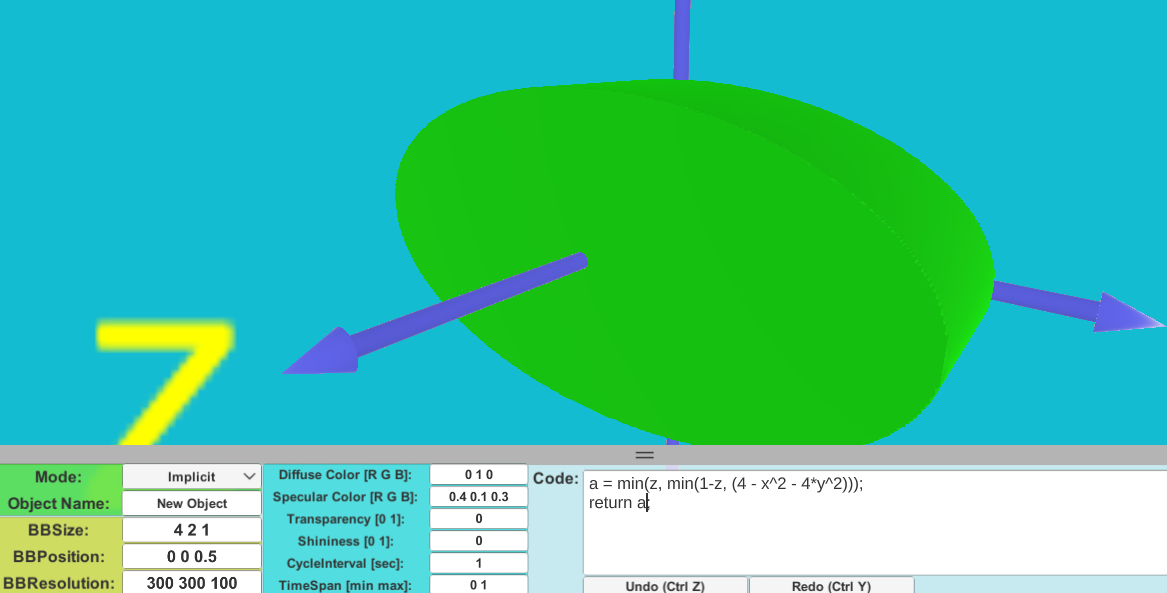
\includegraphics[width=15cm]{fig/q4iic.PNG}
        \centering
    \end{figure}

    However, it is worth noting that this also negatively impacted the rendering time due to to increased amount of 
    rendering points.

\end{homeworkProblem}

\end{document}